% ============================================================
% CHAPTER 5, SECTION 5.2: VIBRATION MONITORING RESULTS
% Every number traces to the raw bench logs (evidence/vibration/VP0x-*/run1.log), re-derived with
% tools/analyse_vib.py and tools/derive_vib_extras.py, or to the V-SIM outputs (VSIM_RECORD.md).
% Figures: figures/fig5_1_sampling.pdf ... fig5_5_fault.pdf, made by figures/fig_5_*.py.
%
% CITATION KEYS TO CHECK before compiling (replace with your own .bib keys):
%   kumar2024  = Kumar and Mandava, ESP32 + MPU9250 bearing study       (your Chapter 2 ref [7])
%   fidali2024 = Fidali et al., MEMS versus piezoelectric sensors         (your Chapter 2 ref [8])
%   chen2024   = Chen et al., wired versus wireless pump monitoring        (your Chapter 2 ref [6])
%   meng2026, ti_sampling = keys already used in Chapter 3.
% Labels assumed from Chapter 3: sec:meth-vib, eq:stop-threshold, app:tests, app:changes, ch:design.
% Items marked [CHECK] need your confirmation.
% ============================================================

\section{Vibration Monitoring Results}
\label{sec:results-vibration}

This section answers the first investigation question of Section~\ref{sec:meth-design}: can the
detector separate normal running, transient disturbance and stoppage on the bench rig? The evidence
is presented in the order in which the detector depends on it. Section~\ref{sec:res-vib-timing}
establishes how often the sensor was actually read and what that means for a rule defined by a count
of samples. Section~\ref{sec:res-vib-baseline} examines the baseline against which every state is
judged, Section~\ref{sec:res-vib-stop} the stoppage and schedule logic, and
Section~\ref{sec:res-vib-faults} the response to disturbances and to loss of the sensor. All bench runs
were run on the same rig in one session, against the baseline of 0.5356~m/s$^2$ recorded in VP01-CAL.
Each result is labelled as a simulation experiment, which tests the decision logic with defined inputs, or
a hardware experiment, which tests the physical sensor chain, and Section~\ref{sec:res-vib-faults} closes
by setting the two against each other.

% ------------------------------------------------------------
\subsection{Acquisition Timing and Window Duration}
\label{sec:res-vib-timing}

Every decision the vibration detector makes rests on a stream of samples, so this subsection first
establishes what that stream can represent and how often it is refreshed. Three results are reported
in turn: the numerical investigation of sampling, filtering and vibration direction (V-SIM-01), the
read interval measured on the bench, and the effect of that interval on the persistence rule that
governs WARNING (V-SIM-02). Together they test the basis of FR-V01, which requires brief and
persistent elevations to be distinguished, and they set the single-module reference for the
combined-load timing in Section~\ref{sec:res-integration-timing}. The third numerical investigation,
on baseline sensitivity, is reported with the baseline results in Section~\ref{sec:res-vib-baseline}.

\paragraph{Simulation experiment V-SIM-01: sampling, filtering and direction.}
Aliasing was expected to be the main risk of sampling at about 45~Hz, but the numerical investigation
shows that it does not threaten an RMS-based indicator. V-SIM-01 sampled an ideal 1~m/s$^2$ sine at
45.27~Hz after one of two illustrative low-pass filter models (Figure~\ref{fig:res-sampling}). With
the 260~Hz model, which corresponds to the filter setting used on the rig, the sampled RMS stayed
within 1.2\,\% of the true RMS at every input frequency from 5 to 100~Hz, including every frequency
above the 22.6~Hz Nyquist limit (Figure~\ref{fig:res-sampling}a). Undersampling relocates such a
component to a false lower frequency~\cite{ti_sampling}, 40~Hz appearing at 5.3~Hz for example, but
it leaves the component's RMS intact. Aliasing would therefore corrupt a spectral analysis but not the
amplitude measure this detector uses. The 21~Hz model, by contrast, reduced the RMS to 0.74 of its
true value at 20~Hz and to 0.27 at 40~Hz, which is consistent with the flat response recorded during
development when the sensor was set to its 21~Hz filter (Appendix~\ref{app:changes}). The choice
between the two settings is the bandwidth trade-off identified for low-cost MEMS sensors in
Chapter~\ref{ch:lit}~\cite{fidali2024}: the narrower filter suppresses aliasing at the cost of the
vibration energy the detector measures, so the wider setting is the appropriate one for an
amplitude-based monitor.

\begin{figure}[H]
\centering
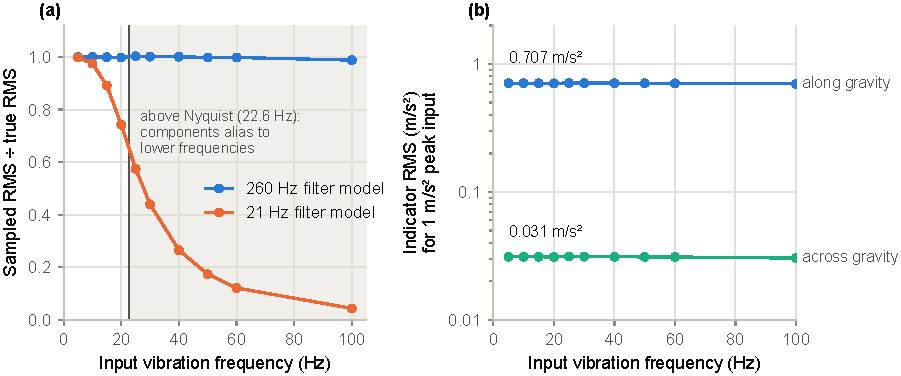
\includegraphics[width=\linewidth]{figures/fig5_1_sampling.pdf}
\caption{Numerical investigation of the vibration indicator (V-SIM-01, \texttt{vibration\_sim.py}): an ideal 1~m/s$^2$ sine sampled uniformly at 45.27~Hz after illustrative
second-order filter models, not a calibrated MPU6050 response. (a)~Sampled RMS relative to the true
RMS for vibration along gravity: aliasing above 22.6~Hz leaves the RMS intact with the 260~Hz model,
whereas the 21~Hz model attenuates it. (b)~Indicator RMS for the same amplitude applied along and
across gravity.}
\label{fig:res-sampling}
\end{figure}

The same investigation exposed a limitation the design had not anticipated: the indicator responds
strongly to vibration along gravity and only weakly to vibration across it
(Figure~\ref{fig:res-sampling}b). The firmware computes the RMS of the deviation of the total
acceleration from gravity. A 1~m/s$^2$ vibration along gravity changes the length of the acceleration
vector directly and gave 0.707~m/s$^2$, whereas the same vibration across gravity mainly rotates the
vector and gave only 0.031~m/s$^2$, about 4\,\% as much. This offers an explanation for an earlier exploratory
observation, that the printed RMS did not appear to rise when the fan speed was changed.
That observation had been attributed to aliasing, which Figure~\ref{fig:res-sampling}a rules out as a
cause of reduced RMS. Two other explanations remain open: the board-mounted arrangement may have
attenuated the vibration reaching the sensor, and the speed log carries no time stamps or speed
markers, so it cannot show whether the RMS rose or not. Directional insensitivity is therefore a
model-supported hypothesis rather than a finding, because the direction of the fan's vibration was not
measured and the filters are illustrative. Its implication for a pump monitor is concrete: the sensor
should be mounted so that the dominant vibration lies along gravity, or the three axes should be
processed separately, which would also permit the spectral analysis that the reviewed bearing study
needed to locate a fault~\cite{kumar2024}.

\paragraph{Hardware measurement: the read interval.}
On the bench, the sensor was read about 10\,\% less often than the firmware's nominal schedule
implies. The main loop waits 20~ms per pass, which would make the 50-sample RMS window 1.0~s and the
6000-sample WARNING history 120~s. Across the 31 one-minute timing windows of the five bench runs,
the mean interval between successful reads was 22.102 to 22.194~ms, the largest single interval was
34.028~ms, and no interval exceeded 50~ms. The work done in each pass therefore added about 2.1~ms to
the delay, lengthening the RMS window to about 1.1~s and the WARNING history to 132.6 to 133.2~s.
These per-read values agree within 0.1~ms with the 22.09~ms loop time measured on earlier firmware and
used in Section~\ref{sec:meth-vib}, so the sampling assumption of the numerical work holds for the
final bench firmware.

\begin{table}[H]
\centering\begingroup\methodtabset
\caption{Effect of the read interval on the WARNING rule (V-SIM-02, \texttt{vibration\_experiment2.py},
synthetic input raised to twice the baseline RMS at 170~s). The measured range is from the 31 timing
windows of the bench experiments.}
\label{tab:vsim-timing}
\begin{tabularx}{\linewidth}{|Q{3.3cm}|Q{2.6cm}|Z|}
\hline
\textbf{Read interval} & \textbf{History length} & \textbf{First WARNING after the rise} \\
\hline
20~ms (nominal delay) & 120.0~s & 60.4~s \\ \hline
22.09~ms (simulated) & 132.5~s & 66.7~s \\ \hline
30~ms (simulated) & 180.0~s & 90.6~s \\ \hline
22.10 to 22.19~ms (measured) & 132.6 to 133.2~s & not tested on hardware \\ \hline
\end{tabularx}
\endgroup
\end{table}

\paragraph{Simulation experiment V-SIM-02: persistence and read interval.}
The lengthened interval matters because the persistence rule is defined by a count of samples rather
than by time. V-SIM-02 reproduced the firmware's RMS, CAUTION and WARNING logic in Python, was checked
by six unit tests that all passed, and was driven with synthetic acceleration raised to twice the
baseline RMS from 170~s. A 5~s elevation produced CAUTION but not WARNING, a sustained elevation
produced WARNING 66.7~s after it began, and an elevation switched on and off every 8~s produced
WARNING after 129.1~s. The rule therefore separates brief from persistent elevation, as FR-V01
requires. Table~\ref{tab:vsim-timing} shows the cost of defining it by count: the delay to WARNING
grows in proportion to the read interval, from 60.4~s at the nominal 20~ms to 90.6~s at 30~ms, so any
additional load on the shared loop slows the alarm by the same proportion.
Section~\ref{sec:res-integration-timing} measures that load with every module enabled.

V-SIM-01 and V-SIM-02 met their expected outcomes and are verified by simulation: they confirm the
decision logic under defined inputs, not the behaviour of the physical sensor chain. On the bench the
read interval was stable, and no interval approached the 50~ms limit later applied to the combined
system. With the sampling and timing basis established, Section~\ref{sec:res-vib-baseline} turns to the
reference against which every vibration state is judged.

% ------------------------------------------------------------
\subsection{Baseline Calibration and Stable Operation}
\label{sec:res-vib-baseline}

Every vibration state is a ratio to the running baseline, so the baseline determines what the
detector calls normal. This subsection reports how the baseline was recorded (VP01-CAL), how the
detector behaved against it during undisturbed running (VP01-STAB), and how strongly the
classification depends on the baseline chosen (V-SIM-03). It closes with the observation that the
rig's running level moved while the baseline stayed fixed. Together these results show how far the
OK and CAUTION side of FR-V01 holds on the bench.

\paragraph{Hardware experiment VP01-CAL: recording the baseline.}
The calibration build recorded a running baseline of 0.5356~m/s$^2$, 109.9~s after its configuration
line was printed, which matches the designed 20~s warm-up and 90~s recording (VP01-CAL). Every later
bench log printed \texttt{baseline=0.5356} in its configuration line, so the value was carried into
the bench builds unchanged and the criterion of no manual adjustment was met. The default of
0.7854~m/s$^2$ compiled into the calibration build is replaced by the measured value and played no
part in the results. The thresholds that follow are 0.643~m/s$^2$ for CAUTION (1.2 times the
baseline) and 0.803~m/s$^2$ for WARNING (1.5 times). The baseline rests on a single 90~s recording,
so its repeatability was not established.

\paragraph{Hardware experiment VP01-STAB: undisturbed running.}
In five minutes of undisturbed running (VP01-STAB, Figure~\ref{fig:res-stability}a), the monitor
printed 1140 status lines: 1114 OK, 26 CAUTION and none WARNING. The criterion of no WARNING was met,
and under the rule fixed in Chapter~\ref{ch:methodology} the 26 CAUTION lines are reported as false
alarms for this rig. Their cause lies in where the threshold sits. The printed RMS had a mean of
0.484~m/s$^2$ and a standard deviation of 0.071~m/s$^2$, so the CAUTION threshold lay only
2.2 standard deviations above normal running and was bound to be crossed by the upper tail of that
variation; the 32 short events logged during the run record those crossings. The printed values are
consecutive snapshots of a rolling RMS rather than independent repeats, so these statistics describe
this run and not the rig in general. All 26 CAUTION lines fell within the first 167~s of the 303~s
run, which suggests that the rig settled after start-up, although that was not tested. The largest
value, 0.727~m/s$^2$, stayed below the WARNING threshold. Because no hardware run elevated the
vibration for long enough, the WARNING side of FR-V01 rests on the simulation of
Section~\ref{sec:res-vib-timing}.

\begin{figure}[H]
\centering
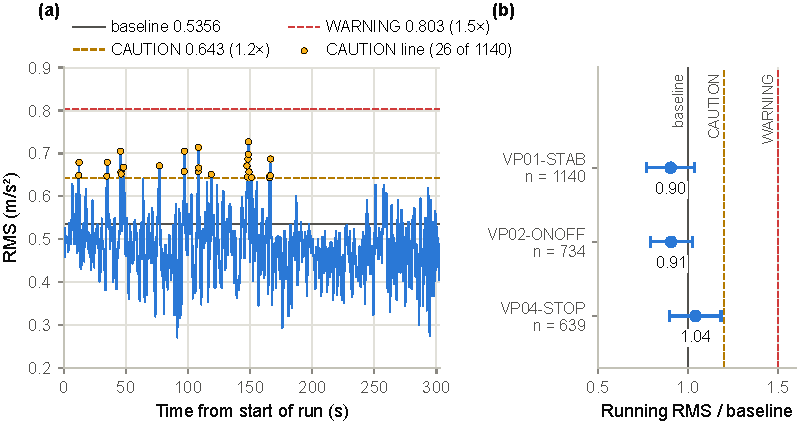
\includegraphics[width=\linewidth]{figures/fig5_2_stability.pdf}
\caption{Baseline stability (baseline 0.5356~m/s$^2$ from VP01-CAL).
(a)~RMS during five minutes of undisturbed running (VP01-STAB, 1140 printed status lines about
250~ms apart), with the 26 lines reported as CAUTION. (b)~Mean running RMS relative to the baseline
in three runs of the same session (dot: mean; bar: one standard deviation of the printed values); running
segments exclude the first 15~s after each switch.}
\label{fig:res-stability}
\end{figure}

\paragraph{Simulation experiment V-SIM-03: baseline sensitivity.}
The third numerical investigation (V-SIM-03) shows why the choice of baseline matters as much as the
measurement itself. The firmware's calibration and classification logic was run twice in simulation,
calibrated once on a synthetic running level of 0.60~m/s$^2$ and once on 1.00~m/s$^2$, and both were
then presented with the same test vibration of 1.10~m/s$^2$. Against the lower baseline the input
was 1.8 times normal, and the detector reported CAUTION after 0.2~s and WARNING after 66.8~s; against
the higher baseline it was 1.1 times normal and produced no alert at all. All three unit tests of
this comparison passed. The result is a property of any baseline-relative detector rather than a
defect: the same vibration is abnormal or normal depending on what was recorded as normal. Its
consequence is that a baseline is only valid while the condition it was recorded under persists.

\paragraph{Comparison across the hardware experiments: running level.}
The bench data show that this condition did not persist even within one session.
Figure~\ref{fig:res-stability}b compares the mean running RMS of three runs made within 40 minutes of
one another on the same rig. The running level was 0.90 of the baseline in VP01-STAB, 0.91 in
VP02-ONOFF and 1.04 in VP04-STOP, where 12.5\,\% of the steady running lines were CAUTION against
1.1\,\% in VP02-ONOFF. With nothing deliberately changed, the level rose by 0.14 of the baseline,
roughly halving its distance from the CAUTION threshold. The cause was not established. The battery
state, the fan's speed setting and the sensor's mounting were not recorded between runs, and VP04-STOP
also used a later build with a revised stoppage threshold, so a change in the rig and a change in the
firmware's output cannot be separated. In the terms of V-SIM-03, the effective baseline moved while
the stored one did not. This is the central limitation of a fixed, once-calibrated reference, and it
agrees with the finding that operating conditions alone can shift RMS levels~\cite{meng2026} and with
the caution in Chapter~\ref{ch:lit} that results from one test bench do not transfer to another
machine or mounting~\cite{kumar2024,fidali2024}. Section~\ref{sec:res-integration-timing} returns to
the same effect at a larger scale, when the running level in the all-modules experiment reached
1.46 times this baseline.

The baseline was therefore recorded as designed, and the detector stayed out of WARNING during
undisturbed running, but a 20\,\% CAUTION margin proved narrow against both the run's own variation
and the drift between runs. VP01-CAL and VP01-STAB met their criteria on hardware, and V-SIM-03 met
its expected outcome in simulation. Section~\ref{sec:res-vib-stop} examines the opposite end of the
scale: whether the detector can tell a motor that has stopped from one that is merely quiet.

% ------------------------------------------------------------
\subsection{Stoppage Detection and Schedule Classification}
\label{sec:res-vib-stop}

A pump that stops during its scheduled running hours is as important to report as one that vibrates
too much, and FR-V02 requires the monitor to tell such a stoppage apart from scheduled inactivity.
This subsection first explains why the original stoppage rule could not work, then reports how the
replacement threshold was set from one run (VP02-ONOFF) and verified on another (VP04-STOP), and
finally examines how the pump window, evaluated against the real-time clock under FR-S01, changes
what the operator is told.

\paragraph{Diagnosis from hardware data: the original stoppage rule.}
The original rule could never have fired, and the reason lies in the indicator rather than the
threshold. It reported STOPPED when the RMS fell below half of the baseline. With the motor stopped,
however, the RMS did not approach zero: after the 15~s allowance it averaged 0.324~m/s$^2$ in
VP02-ONOFF (565 lines) and 0.317~m/s$^2$ in VP04-STOP (1074 lines). Half of the final baseline is
0.268~m/s$^2$, and half of the 0.3476~m/s$^2$ baseline in use when the rule was written is
0.174~m/s$^2$, so with either baseline the resting RMS stayed above the trigger. The logs show where
this floor comes from. At rest the sensor reported a total acceleration of 10.11 to 10.12~m/s$^2$ in
every stopped segment of VP04-STOP, against the 9.8~m/s$^2$ that the firmware subtracts as gravity,
and the spread of the same samples was only about 0.03~m/s$^2$ (Figure~\ref{fig:res-spread}). Because
the square of the RMS equals the square of the mean plus the square of the spread, the resting RMS was
almost entirely this constant offset of about 0.31~m/s$^2$, most likely a gain error of the clone
sensor. No rule based on the RMS level can separate a stopped motor from a fixed offset, whereas the
spread subtracts the mean and keeps only the fluctuation that a running motor produces. The spread
belongs to the same family of time-domain statistics as the RMS and kurtosis used in the reviewed
bearing study~\cite{kumar2024}, and it was adopted as the measure of stoppage.

\begin{figure}[H]
\centering
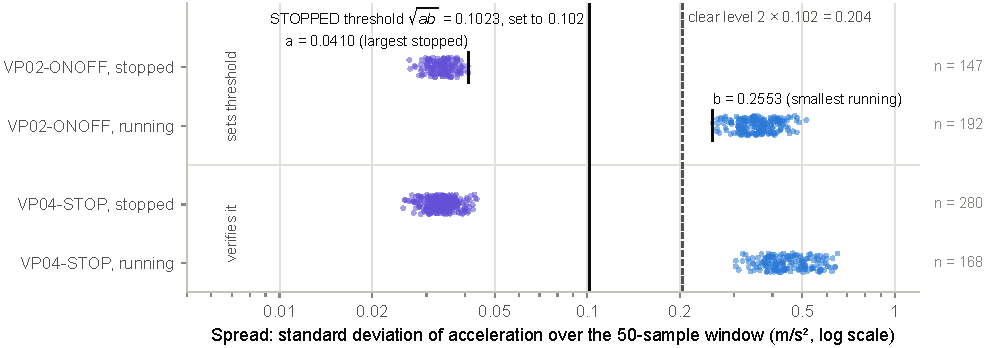
\includegraphics[width=\linewidth]{figures/fig5_3_spread.pdf}
\caption{Spread of acceleration over the 50-sample window, one value per second, with the motor
stopped and running. VP02-ONOFF set the threshold by
Equation~\ref{eq:stop-threshold}; VP04-STOP is a separate later run on the frozen threshold. The
first 15~s after each switch are excluded.}
\label{fig:res-spread}
\end{figure}

\paragraph{Hardware experiments VP02-ONOFF and VP04-STOP: setting and verifying the threshold.}
The threshold was set from VP02-ONOFF by the rule fixed in Chapter~\ref{ch:methodology}. The largest
stopped spread was $a = 0.0410$~m/s$^2$ (147 values) and the smallest running spread
$b = 0.2553$~m/s$^2$ (192 values), so the two sets did not overlap and $b$ exceeded $a$ by a factor
of 6.2. Equation~\ref{eq:stop-threshold} gave $\sqrt{ab} = 0.1023$~m/s$^2$, which was frozen at
0.102~m/s$^2$ in the firmware used for every later run. This separation explains the choice of
threshold but cannot confirm it, because the same data produced it. Confirmation comes from
VP04-STOP, a separate run in which the threshold was not recalculated. There the stopped spread
ranged from 0.0252 to 0.0438~m/s$^2$ (280 values) and the running spread from 0.3038 to
0.6499~m/s$^2$ (168 values). The nearest stopped value lay a factor of 2.3 below the threshold and the
nearest running value a factor of 3.0 above it, so the frozen threshold separated the two states in
new data with a clear margin on both sides.

\begin{figure}[H]
\centering
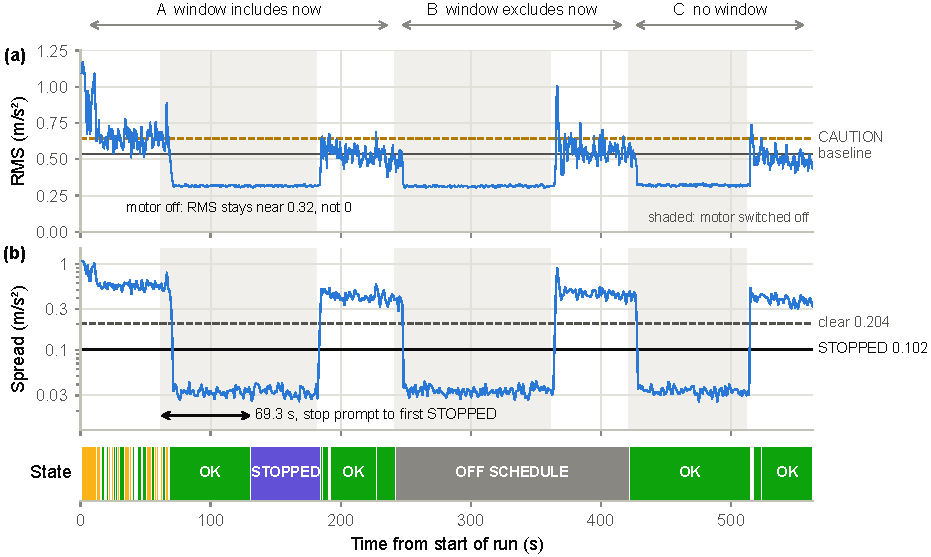
\includegraphics[width=\linewidth]{figures/fig5_4_vp04.pdf}
\caption{Stoppage and schedule verification (VP04-STOP, threshold 0.102~m/s$^2$).
(a)~RMS on an axis from zero, so that the resting level of about 0.32~m/s$^2$ with the motor off is
visible; (b)~spread on a logarithmic axis with the STOPPED threshold and the clear level; (c)~reported
state. Phases: A, the pump window includes the current clock time; B, it excludes it; C, no window is
set. Shaded intervals: motor switched off. The rapid alternation at the start of phase~A is CAUTION
and OK lines during the raised running level of this run. The last STOPPED line was printed 2.5~s
after the switch-on prompt in phase~A.}
\label{fig:res-vp04}
\end{figure}

\paragraph{Hardware experiment VP04-STOP: stoppage timing and schedule classification.}
The timing of the STOPPED report in phase~A follows the design closely (Figure~\ref{fig:res-vp04}).
The first STOPPED line came 69.3~s after the stop prompt. The spread fell below the threshold 9.8~s
after the prompt, an interval that contains the operator's reaction and the motor's run-down, and
STOPPED followed 59.6~s later, which matches the 60~s confirmation hold within the 1~s resolution of
the spread output. A stoppage is therefore reported about a minute after the motor stops, by design.
While the hold elapsed the monitor continued to report OK, with 14 CAUTION lines in the first 6.4~s
as the motor ran down, which accounts for the 247 OK and 14 CAUTION lines in the stopped segment of
Table~\ref{tab:res-vp04}. The 135 CAUTION lines in the running segments of phase~A reflect the raised
running level of this run reported in Section~\ref{sec:res-vib-baseline}, not the stoppage logic.

\begin{table}[H]
\centering\begingroup\methodtabset
\caption{Reported states in VP04-STOP by phase and motor condition (counts of printed status lines).
Criteria from Appendix~\ref{app:tests}.}
\label{tab:res-vp04}
\begin{tabularx}{\linewidth}{|Q{2.4cm}|Q{1.6cm}|Z|Q{2.9cm}|}
\hline
\textbf{Phase} & \textbf{Motor} & \textbf{Reported states} & \textbf{Criterion} \\
\hline
A: window includes now & stopped & STOPPED 192, OK 247, CAUTION 14 & Partly met: 10 STOPPED lines after switch-on \\
 & running & OK 305, CAUTION 135, STOPPED 10 & \\ \hline
B: window excludes now & stopped & OFF SCHEDULE 451, OK 1 & Met: no STOPPED \\
 & running & OFF SCHEDULE 227 & \\ \hline
C: no window & stopped & OK 339 & Met: no STOPPED \\
 & running & OK 181, CAUTION 7 & \\ \hline
\end{tabularx}
\endgroup
\end{table}

Phase~A nevertheless missed its strict criterion. Ten STOPPED lines followed the switch-on prompt, the
last 2.5~s after it, so STOPPED was reported while the motor was, by the script, running. The cause is
visible in the log. The firmware clears STOPPED only when the spread rises above 0.204~m/s$^2$, twice
the threshold, and the spread was 0.028~m/s$^2$ at 0.7~s after the prompt and 0.305~m/s$^2$ at
2.8~s, so it crossed the clear level between those times, consistent with the last STOPPED line at
2.5~s. The ten lines are the time the motor took to spin up and the clear rule took to respond, not a
misclassification of a running motor. Applying the 15~s switching allowance defined for VP02-ONOFF
would remove them, but that allowance was not written for VP04-STOP and is not applied after the
fact, so phase~A is reported as partly met. A future protocol should state a switching allowance for
every stop and start test.

Phases~B and~C met their criteria, and phase~C exposes a consequence worth stating plainly. Outside
the window the monitor reported OFF SCHEDULE throughout, stopped and running alike, and never STOPPED,
so an expected stoppage was not raised as a fault. With no window set, stoppage detection was off by
design, and the stopped motor was reported as OK in all 339 lines. ``OK'' therefore means ``no
abnormal vibration'' rather than ``running'', and an operator who has not set a pump window receives
no indication that the pump has stopped; Section~\ref{sec:res-integration-reporting} returns to this as
a question of what the interface tells the operator. Two further limits apply. The window was evaluated
against the board's real-time clock, which was then 30~h~58~min behind true time, so the schedule
logic was tested against the clock's own time of day rather than calendar time. All results come from
one motor at one speed, so the threshold applies to this rig and mounting only.

VP02-ONOFF therefore met its criterion and produced a threshold that separated stopped from running
with a factor of two to three in margin on new data, and VP04-STOP met the schedule criteria of
phases~B and~C on hardware, with phase~A partly met. FR-V02 is supported on the bench for one motor,
subject to the clock and switching limits above. Section~\ref{sec:res-vib-faults} turns from the motor
to the sensor: what the monitor reports when the vibration is disturbed or the sensor itself fails.

% ------------------------------------------------------------
\subsection{Disturbances, Sensor Faults and Event Records}
\label{sec:res-vib-faults}

The final group of experiments moves away from steady running to the conditions that test whether
the monitor can be trusted: a disturbance it should not over-react to, a sensor that stops answering,
and the record it keeps of what happened. These address FR-V01 for short disturbances, FR-S04 for a
failed sensor, FR-S05 for whether one failing module stalls the shared loop, and FR-V03 for event
retention. The subsection closes by setting every simulation prediction made in this section against
the hardware experiment that tested it.

\paragraph{Hardware experiment VP03-DIST: hand-applied disturbances.}
This experiment was a characterisation with no pass criterion, because the force of a hand tap cannot
be controlled. The taps produced 57 events and a largest printed RMS of 6.151~m/s$^2$, more than
eleven times the baseline, yet no WARNING was reported at any point: the disturbances escalated to
CAUTION and no further. The experiment also exposed a procedural weakness. The strongest response,
62 non-OK lines and 23 events, fell in the interval that the script labelled as running between the
brief and sustained taps, while the scripted sustained interval showed only 14 non-OK lines. The taps
and the prompts were therefore out of step, so neither the delay from a disturbance to its report nor
the time to return to OK can be measured from this run. A repeat would need the tap times recorded,
for example by a second sensor or a video.

\paragraph{Hardware experiment VP05-FAULT: sensor loss during a run.}
The firmware rejected every reading for a configured 5~s, and the monitor reported SENSOR ERROR
instead of a stale state (Figure~\ref{fig:res-fault}). SENSOR ERROR appeared 2.05~s after the
injection started, against a designed timeout of 2.00~s, and normal reporting resumed 1.04~s after it
ended, against a designed recovery of 1.00~s. The clock continued to print throughout with no gap
longer than 1.07~s, so the failure of the vibration sensor did not stall the loop that the clock
shares, which is the single-module evidence for FR-S05. After recovery the RMS restarted from
0.004~m/s$^2$, because the firmware clears the RMS window and the WARNING history rather than resume
from values recorded before the failure. The excess over the designed times, 38 to 60~ms, is larger
than one loop pass of at most 34~ms, so part of it is attributed to the laptop's time stamping of the
serial lines; this was not confirmed. The fault was injected in firmware, not by disconnecting a wire
from a running board, so the electrical behaviour of a physical fault was not tested.

\begin{figure}[H]
\centering
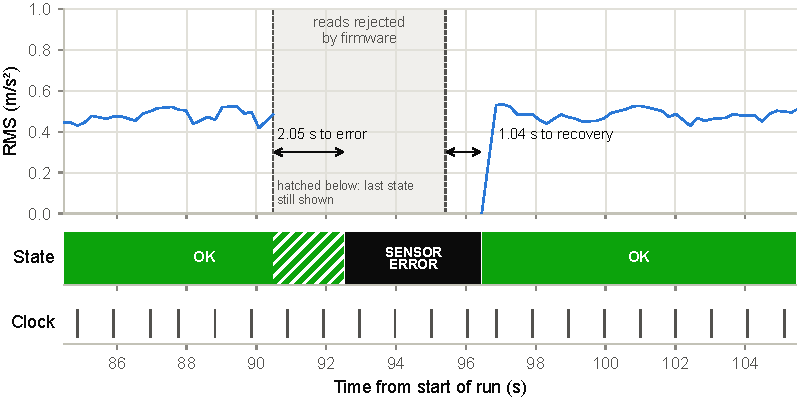
\includegraphics[width=\linewidth]{figures/fig5_5_fault.pdf}
\caption{Firmware-injected sensor loss (VP05-FAULT, build \texttt{esp32doit-bench-fault}). Shaded:
every reading rejected for a configured 5~s. Hatched: interval in which the last printed state was still
shown, before the SENSOR ERROR line. Clock: lines printed by the real-time clock module, one per second.}
\label{fig:res-fault}
\end{figure}

\paragraph{Hardware experiment VP05-NOSENSOR: start-up without the sensor.}
With the sensor disconnected before power-up, SENSOR ERROR was reported 0.47~s after the first logged
line, the board did not hang, and the clock printed 91 lines in 92.9~s, so three of the four criteria
were met. The fourth, a retry about every 5~s, could not be observed. The bus library printed 3189
read-error lines, 34 per second, because the firmware attempts a read on every pass of the loop, and
any periodic re-initialisation was hidden in that output. The same flood of error lines would fill a
serial log quickly in service, so a rate-limited retry with its own log line is a necessary
refinement.

\paragraph{Hardware analysis VP06: event records.}
Across all seven bench logs the firmware recorded 242 vibration events, none of which reached
WARNING. In 241 of them the duration was a whole multiple of 22.11~ms to within a quarter of a period,
which confirms that event timing is quantised by the read interval measured in
Section~\ref{sec:res-vib-timing}. Each event carried a time stamp, a duration and a peak RMS, and the
time stamps increased monotonically, but they were 30~h~58~min behind true time because of the clock
error. The firmware keeps only the last ten events in memory and prints them to the serial port; they
are not served to the operator interface, and the 24-hour summary designed for that purpose was not
implemented in the firmware. An event that is not read before ten newer ones replace it is lost, the
same weakness that the reviewed pump study found in intermittent data collection, which missed
short-duration events~\cite{chen2024}. FR-V03 is therefore met only in part: events are generated and
stamped, but not retained for later review.

\paragraph{Simulation against hardware.}
Table~\ref{tab:res-vib-validation} sets each prediction of the numerical investigations against the
hardware experiment that tested it. Where both exist they agree: brief disturbances stopped at CAUTION
in simulation and on the rig, the failure mode exposed in simulation was removed and the fix confirmed
on hardware, and the dependence on the baseline predicted by V-SIM-03 appeared on the bench as drift.
Two predictions remain untested on hardware: the time to WARNING under a sustained elevation, which no
planned hardware experiment produced, and the insensitivity to vibration across gravity, because the
direction of the rig's vibration was never measured. The stoppage rule is the reverse case: it was
designed and verified on hardware alone, because the firmware modelled in simulation did not yet
contain it.

\begin{table}[H]
\centering\begingroup\methodtabset
\caption{Simulation predictions set against the hardware experiments that tested them.}
\label{tab:res-vib-validation}
\begin{tabularx}{\linewidth}{|Q{4.0cm}|Z|Q{2.6cm}|}
\hline
\textbf{Simulation prediction} & \textbf{Hardware result} & \textbf{Agreement} \\
\hline
V-SIM-02: a brief elevation reaches CAUTION but not WARNING & VP03-DIST: taps up to 11.5 times the baseline gave CAUTION, never WARNING & Agrees (taps uncontrolled) \\ \hline
V-SIM-02: failed reads leave the last state on display & VP05-FAULT, after the SENSOR ERROR state was added: error reported after 2.05~s & Defect found in simulation, fix confirmed on hardware \\ \hline
V-SIM-02: time to WARNING grows with the read interval & Read interval 22.10 to 22.19~ms, matching the simulated 22.09~ms & Agrees for the interval; WARNING not produced in a planned run \\ \hline
V-SIM-03: the outcome depends on the baseline & Running level moved from 0.90 to 1.04 of a fixed baseline & Same mechanism observed \\ \hline
V-SIM-01: little response to vibration across gravity & Direction of the rig's vibration not measured & Not tested \\ \hline
\end{tabularx}
\endgroup
\end{table}

\begin{table}[H]
\centering\begingroup\methodtabset
\caption{Summary of the vibration experiments against the criteria fixed in
Chapter~\ref{ch:methodology}.}
\label{tab:res-vib-summary}
\begin{tabularx}{\linewidth}{|Q{2.1cm}|Q{1.6cm}|Z|Q{3.2cm}|}
\hline
\textbf{Experiment} & \textbf{Type} & \textbf{Key result} & \textbf{Criterion} \\
\hline
V-SIM-01, 02, 03 & Simulation & RMS preserved under aliasing; 4\,\% response across gravity; brief elevation stops at CAUTION; outcome depends on the baseline & Expected outcomes met; 9 unit tests pass \\ \hline
VP01-CAL & Hardware & Baseline 0.5356~m/s$^2$ after 109.9~s & Met \\ \hline
VP01-STAB & Hardware & No WARNING; 26 of 1140 lines CAUTION & Met; CAUTION reported as false alarms \\ \hline
VP02-ONOFF & Hardware & $a = 0.0410$, $b = 0.2553$, threshold 0.102~m/s$^2$ & Met \\ \hline
VP04-STOP & Hardware & STOPPED after 69.3~s; separation held on new data & A partly met; B and C met \\ \hline
VP03-DIST & Hardware & Peak 6.151~m/s$^2$, no WARNING & Characterisation \\ \hline
VP05-FAULT & Hardware & SENSOR ERROR at 2.05~s, recovery at 1.04~s, clock unbroken & Met (injected fault) \\ \hline
VP05-NOSENSOR & Hardware & SENSOR ERROR at 0.47~s, no hang & 3 of 4 met; retry not observable \\ \hline
VP06 & Hardware & 242 events, stamped, quantised at 22.11~ms & Partly met: not retained for review \\ \hline
\end{tabularx}
\endgroup
\end{table}

Taken together (Table~\ref{tab:res-vib-summary}), the simulation and hardware experiments establish
that on this rig the detector separates a running motor from a stopped one with a clear margin on new
data, keeps brief disturbances from escalating to WARNING, distinguishes an expected stoppage from an
unexpected one when a pump window is set, and reports a failed sensor rather than a stale state. They
do not establish that the detector would recognise a mechanical fault: no fault was introduced,
WARNING was not reached in any planned hardware experiment, and the reviewed studies show that even a
rising RMS indicates that something has changed without identifying what~\cite{kumar2024}. The
experiments also exposed two limits the design did not anticipate, a running level that drifts against
a fixed baseline and an indicator that is largely insensitive to vibration across gravity.
Section~\ref{sec:results-water} turns to the water-quality module, where the corresponding question is
whether the readings themselves can be trusted.
